\documentclass[12pt]{article}
\usepackage[utf8]{inputenc}
\usepackage{graphicx}

\title{High-level error monitoring for a domain-oriented microservices architecture gateway}
\author{Cristian Manuel Abrante Dorta}
\date{\today}

\begin{document}

\maketitle

\section{Introduction}

Over the past few years, there has been debate on how to properly organize and deploy service-oriented architectures. One of the software architecture patterns that has gained the most popularity today is microservices \cite{MicroservicesAdoption}. Many large, medium and even small software companies have adopted this architecture because of its enormous benefits compared to traditional, monolithic software applications.\\

Microservices are an extension of service-oriented architecture. The main objective is that each of these microservices provides a well-defined and clear scope of functionalities, which can be accessed by another microservice using \textit{remote procedure calls} \cite{nelson1981remote}. The main advantage of this pattern is that it can be established clear ownership of each microservice by different teams where they are responsible for the development, maintenance, and deployment. This is a clear advantage over the classic monolithic architecture, since in these, although the development tasks may be divided among different teams, the deployment of a single functionality involves the deployment of the entire system, which is then prone to cause major problems that can lead to the complete shutdown of the application.\\

Although the microservices architecture represents a step forward in the design of software systems, it also has some drawbacks compared to monolithic architectures, such as performance. In a traditional monolithic application subroutine calls are something that can be solved within the same process and machine, however, in microservices, the call has to be made over the network, which is something that may eventually introduce some execution delays. Apart from this, there is another problem faced by microservices architectures, which is the orchestration of thousands of different microservices, when dealing with enterprises operating on a large scale. In this case, any problem caused by one microservice can spread across many of them, and engineers have to debug calls coming from a huge stack of different services, which is something that can be challenging and time-consuming.\\

In order to provide an scope that would simplify the maintenance of the microservices set, many companies had adopted the \textbf{Domain Oriented Microservices Architecture} pattern \cite{DOMAUber}. Using this architecture, many microservices can be grouped within a logical division, called Domain, that fits the needs of the enterprise. To isolate the domains and make them easier to maintain and debug, one approach which can be applied is to create a common gateway that exposes the domain's interface (usually as routes that can be called with different HTTP methods). Apart from being the single point of entry for specific domains, the gateway can also provide different high-level responsibilities, such as authentication, routing, rate limiting, load balancing, etc. This pattern has been widely adopted by companies operating on a large scale, such as Uber \cite{GatewayUber} or Unity Technologies (Figure \ref{fig:unity-acquire-domain}).\\

\begin{figure}[h]
    \centering
    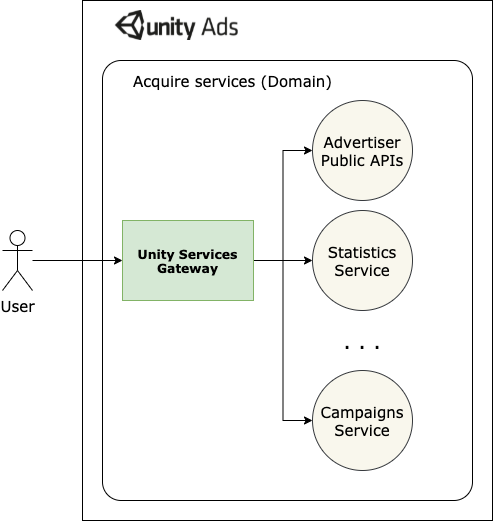
\includegraphics[scale=0.3]{src/proposal/img/unity-services-diagram.png}
    \caption{Domain-oriented microservices architecture structure in Unity Technologies}
    \label{fig:unity-acquire-domain}
\end{figure}

The gateway is in itself another microservice, consequently the error monitoring of it is a crucial task for maintenance the overall health of the system. About microservices logging and monitoring there is already a well established action framework \cite{MicroservicesBestPractices}, which can be summarized as the storage of a log entry in a centralized server (for example Google Cloud or Amazon Web Services) for each request or error that it is produced in the system. Usually that is enough for tracing back each of the requests that the system is receiving.\\

In the particular case of the \textbf{Unity Services Gateway}, which is the entry point of the acquire domain of Unity technologies, there are some questions raised about the high-level responsibilities of the gateway by project managers or some development teams, such as: \textit{what users or organizations are hitting our rate limits?} \textit{What is the amount and frequency of authentication errors our system is having?}.\\

The answers to those questions are relevant because some actions can be taking against malicious users which are doing too many queries to the system or directly some organizations can be contacted to check if their integration with the APIs that the company provides are working properly. Nevertheless, the current log setup, which is the classical microservices logging framework \cite{MicroservicesBestPractices}, is not enough for answering those questions. This is mainly due to the fact that the current log events only store the minimal piece of information required to trace back the request but do not contain complex fields, such as organization ids, paths for the request, rate limit quotas exceeded, etc.\\

One might think that simply by extending the logs entry to contain more information is enough for solving this problem, nevertheless this simple approach is not effective due to some reasons. The first one is that the data needed for solving those questions has to be extracted from different sources, which is something that it is reasonable to do when dealing with errors but can not be generalized to all logs entries as would dramatically increase the processing time of the requests in a system that is receiving thousands of request per seconds. The second reason is that the logging tool is shared among many microservices, so none of them has to worry in how to communicate with the cloud provider, this is why it is better to keep simple the amount of fields that the logs are storing. The final reason is the single responsibility principle, as it seems sensible to separate the data store that would keep complex error fields that would solve high-level questions from the actual log registry that would keep track of the requests.\\

Taking this into account, the objective of this thesis can be defined as determine the best way to monitor the errors produced by the high-level responsibilities of a Domain Oriented Microservice Architecture gateway. \\

\section{Research questions}
\label{sec:research-questions}

In order to achieve the objective, three different research questions are formulated, used as the guiding thread for the research.

\begin{itemize}
    \item[\textbf{Q1}] \textit{What is the best way to represent the possible high-level errors that a domain-oriented architecture gateway can produce?}
    \item[\textbf{Q2}] \textit{What is the optimal technology for storing the errors that a domain-oriented architecture gateway can produce?}
    \item[\textbf{Q3}] \textit{How to correctly visualize and communicate with the stakeholders the errors a domain-oriented architecture gateway can produce?}
\end{itemize}

\section{Expected outcomes}

Based on the research questions defined in Section \ref{sec:research-questions}, it is important to state which are the expected outcomes that are going to be produced with the thesis and which is the intended plan for producing those results and hence solve the research questions. First of all, it is important to state that all the experiments are going to be conducted using the Unity Services Gateway as an example of domain oriented architecture gateway.\\

The list of expected outcomes is:

\begin{itemize}
    \item \textbf{Requirements analysis}: In order to determine the best way for representing the high-level errors of a domain-oriented architecture gateway, and thus addressing \textbf{Q1}, a requirements analysis is going to be performed. In order to do that, the first step would be to identify the stakeholders of the project, which preliminarily are the project managers of the developed software services and the development team, and interview them to find out what are the high-level questions related to gateway monitoring that cannot be answered with the current configuration. Using the information of those interviews, the requirement analysis is going to be produced.
    \item \textbf{Software design}: Having the requirements analysis as a base, the next outcome would be the software design. This design will include the error events structure that will contain all the necessary information for addressing the questions of the stakeholders as well as a high level design of the software system that will address the problem.
    \item \textbf{Data source comparison and evaluation}: To solve \textbf{Q2}, it is crucial to establish what are the criteria for the definition of the optimal storage technology. Initially, the criteria are: the complexity of the aggregation (since the data has to be composed of different data sources), the cost per insertion, storage and access (since the data source could insert and store thousands of records) and, finally, the integration with the current technological configuration. The expected outcome is the comparison between different databases (RDBMS, NO-SQL and data warehouse) in the context of the events storage.
    \item \textbf{Prototype implementation}: having performed the software design and also having done the selection of the ideal data source for our use case, the next expected outcome would be the implementation of a prototype for the particular case of the Unity services gateway. For doing that, the source code of the gateway has to be modified in order to gather the information for the events, and there are some architectural changes that has to be done in order to store those events in the selected data source.
    \item \textbf{Custom visualization tool (Grafana dashboard)}: In order to solve \textbf{Q3} a custom Grafana dashboard is going to be developed in order to map the data sources with the visual representation that will easily solve the high-level questions of the stakeholders.
\end{itemize}

\bibliographystyle{plain}
\bibliography{proposal}

\end{document}
